\documentclass{article}
\usepackage{geometry}
\usepackage{paralist}
\usepackage[T1]{fontenc}
\usepackage{reledmac}
\usepackage{changepage}
\usepackage{layout}

\usepackage{pgfplots}
\usepackage{tikz}
\usetikzlibrary{positioning}
\usetikzlibrary{shapes.geometric, arrows}
\usetikzlibrary{calc, shapes, backgrounds}
\tikzstyle{arrow} = [thick,->,>=stealth]

\usepackage{graphicx} 
\graphicspath{ {./images/} }

\usepackage{fancyhdr}
\fancyhead[L]{
	\begin{tabular}{l}
		\Large \textbf{\textsc{Distributed Systems}} \\
		\large Project 02 - Part 01
	\end{tabular}
}
\fancyhead[R]{
	\begin{tabular}{r}
		16-124-836 \\
		Marcel \textsc{Zauder}
	\end{tabular}
}
\renewcommand{\headrulewidth}{0.4pt}
\fancyfoot[C]{\thepage}
\renewcommand{\footrulewidth}{0.4pt}
\setlength{\headsep}{35pt}
\setlength{\textheight}{600pt}

\usepackage{hyperref}

\begin{document}
	\pagestyle{fancy}
	
	All required files are in their respective directories with specified names.	
	
	\section*{Task 04 - Simple point-to-point topology, \texttt{ping} and \texttt{perf}}
	\begin{adjustwidth}{2em}{2em}
		The average round trip delay time is approximately 0.043 ms, therefore the one-way latency time is approximately 0.0215ms.
	\end{adjustwidth}
	
	\section*{Task 05 - Bandwidth sharing}
	\begin{adjustwidth}{2em}{2em}
		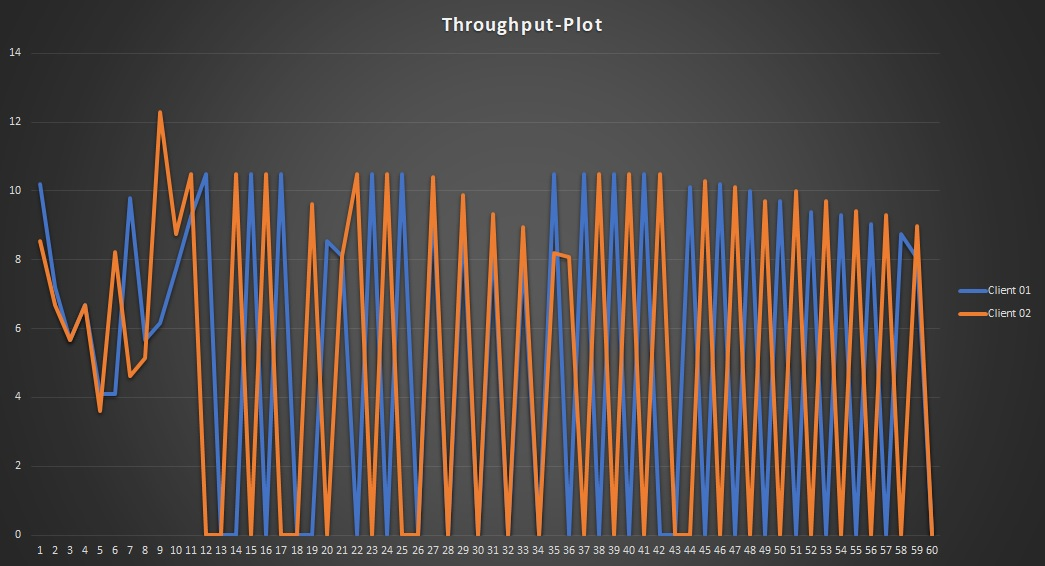
\includegraphics[scale=0.5]{Plot.jpg} \\
		As one can see after some time the clients are sending alternately their data to the server. In the beginning the switch tries to  find the best possible way to handle the incoming requests from the clients. This leads to a very messy transmission rate because there is only a limited amount of bandwitdh which each of the clients wants all for themself. The little part where both clients send synchronously could have happened because it was not really possible to start both clients at the exact same time so this can be explained by rounding errors. In total one client is sending at one time and then waits for the other client to send their request therefore we see these alternating graphs between $\sim$ 10 Mbit/s (the bandwidth of the link) and 0 Mbit/s.
	\end{adjustwidth}
\end{document}